\chapter{Theory}
\label{chap:theory}

In this chapter, we give a theoretical introduction to the topic dealt with in this thesis. The ultimate goal of this chapter is to introduce and describe analytical models for subsurface scattering. First, we will give a brief introduction to the nature of light, and how we physically describe it. Secondly, we will introduce the basic radiometric quantities that will be used throughout the chapter. Then, we will describe how this quantities are related and can be used to describe light-material interaction, using reflectance functions, of which BSSRDF functions are a special case. Finally, we will introduce subsurface scattering and the diffusion approximation, concluding with a description of two BSSRDF models, by \cite{Jensen:2001:PMS:383259.383319} and \cite{IMM2013-06646}.


\renewcommand{\arraystretch}{1.2}
\begin{table}[!ht]
\rowcolors{2}{white}{myblue}
\begin{tabular}{|l|l|}
\hline
Quantity                           & Description                                             \\ %\hline
$\mathbf{x}$                       & Point, not normalized vector                            \\ %\hline
$(x_x,x_y,x_z)$                    & Components of a vector                                  \\ %\hline
$\vec{\omega}$                     & Normalized vector, direction                            \\ %\hline
$Q$                                & Radiant Energy                                          \\ %\hline
$\Phi$                             & Radiant Flux                                            \\ %\hline
$E$                                & Irradiance                                              \\ %\hline
$I$                                & Intensity                                               \\ %\hline
$L$                                & Radiance                                                \\ %\hline
$\vec{n} \cdot \vec{m}$            & Dot product between two vectors                         \\ %\hline
$\vec{n} \times \vec{m}$           & Cross product between two vectors                       \\ %\hline
$A$                                & Area                                                    \\ %\hline
$i$ (subscript)                    & Denotes incoming direction or incidence point           \\ %\hline
$o$ (subscript)                    & Denotes outgoing direction or exitance point            \\ %\hline
M (capital letter)                 & Denotes matrix (see Appendix A)                         \\ %\hline
$f(...)$                           & BRDF function                                           \\ %\hline
$S(...)$                           & BSSRDF function                                         \\ %\hline
$\eta = \frac{n_1}{n_2}$           & Relative index of refraction                            \\ %\hline
$R(\eta,\vec{\omega})$             & Fresnel reflection term                                 \\ %\hline
$T(\eta,\vec{\omega})$             & Fresnel transmission term                               \\ %\hline
$\vec{\nabla} \cdot \vec{x}$       & Directional derivative of vector $\vec{x}$              \\ %\hline
$\sigma_a$                         & Absorption coefficient                                  \\ %\hline
$\sigma_s$                         & Scattering coefficient                                  \\ %\hline
$g$                                & Mean cosine coefficient                                 \\ %\hline
$\sigma_t = \sigma_s + \sigma_a$   & Extinction coefficient                                  \\ %\hline
$\sigma'_s = \sigma_s (1-g)$       & Reduced scattering coefficient                          \\ %\hline
$\sigma'_t = \sigma'_t + \sigma_a$ & Reduced extinction coefficient                          \\ %\hline
$\sigma_{tr}$                      & Transmission coefficient                                \\ %\hline
$\alpha'$                          & Reduced albedo                                          \\ %\hline
$\cs$                              & Approximation of the scalar fluence Fresnel integral    \\ %\hline
$\ce$                              & Approximation of the vector irradiance Fresnel integral \\ \hline
\end{tabular}
\caption{Table of the notation used in this thesis.}
\end{table}
\FloatBarrier

\section{Light and Radiometry}
Light is a form of electromagnetic radiation, that propagates through space as a sinusoidal wave. Usually by \emph{light} we refer to \emph{visible light}, the small part of the electromagnetic spectrum the human eye is sensible to (see Figure \ref{fig:spectrum}). This small window is between the \SI{380}{\nano\meter} of infrared and \SI{750}{\nano\meter} of ultraviolet light, but the precise boundaries may vary according to the environment and the observer. Instead explicitly noted, we will use the terms light and visible light interchangeably in this report.

The study of light is usually referred as \emph{optics}. In computer aided image synthesis, we are interested in representing faithfully how visible light propagates how it interacts with the objects and the materials in a scene. In addition, we are interested in lighting effects that are noticeable at human scales (\SI{1}{\milli\meter} - \SI{1}{\kilo\meter}), like subsurface scattering, absorption and emission phenomena. Optics studies more effects, like diffraction, interference and quantum effects, but we are not interested in representing them because for visible light they happen on a microscopic scale (\SI{1}{\nano\meter} - \SI{1}{\micro\meter}). 

\begin{figure}[!ht]
\centering
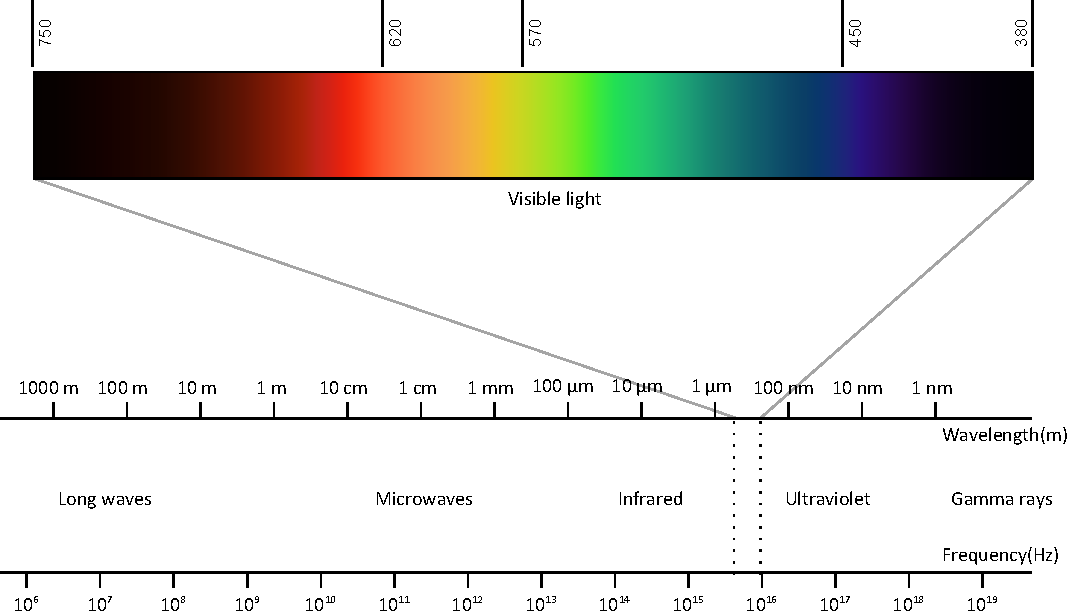
\includegraphics[width=1.0\textwidth]{images/spectrum.pdf}
\caption{The electromagnetic spectrum.}
\label{fig:spectrum}
\end{figure}

The branch of physics that studies how to measure electromagnetic radiation is called \emph{radiometry}. The energy of light, like all the others forms of energy, is measured in \emph{Joules} [\si{\joule} $=$ \si{\kg\meter\square\per\second\square}], and its power in \emph{Watts} [\si{\watt} $=$ \si{\kg\meter\square\per\second\cubed}]. \emph{Photometry}, on the other hand, measures electromagnetic radiation as it is perceived from the human eye, and limits itself only to the visible spectrum, while radiometry spans all of it. The corresponding names for energy and power in photometry are \emph{radiant energy}, measured in \emph{talbots} [\si{\candela\second}], and \emph{radiant flux}, measured in \emph{candelas} [\si{\candela}]. 

In image synthesis it is more common to use radiometry, as its quantities directly derive from the electromagnetic theories, are universal, and can be easily converted to the photometric ones when necessary. The most important radiometric quantities used in computer graphics are \emph{radiant flux}, \emph{radiant energy}, \emph{radiance}, \emph{irradiance} and \emph{intensity}.

\section{Radiometric quantities}

\subsection{Radiant flux}
The radiant flux, also known as radiant power, is the most basic quantity in radiometry. It is usually indicated with the letter $\Phi$ and it is measured in joules per seconds [\si{\joule\per\second}] or Watts [\si{\watt}]. The quantity indicates how much power the light irradiates per unit time. 

\subsection{Radiant energy}
Radiant energy, usually indicated as $Q$, is the energy that the light carries in a certain amount of time. Like all the other SI units for energy, it is measured in joules [\si{\joule}]. Radiant energy is obtained integrating the radiant flux along time for an interval $\Delta T$:

$$
Q = \int_{\Delta T} \Phi(t) \; dt
$$

Due to the dual nature of the light, the energy carried by the light can be derived both considering light as made of particles, called \emph{photons}, or considering it as a wave. We will not dig further into the topic, because for rendering purposes is not important if we characterize light as a flux of particles or as a sinusoidal wave.

\subsection{Irradiance}

Irradiance, usually defined as $E$, is the radiometric unit that measures the radiant flux per unit area \emph{falling} on a surface. It is measured in Watts per square meter [\si{\watt\per\square\meter}]. It is defined as the flux per unit area:
$$
E = \frac{d\Phi}{dA}
$$
Irradiance is usually the term in literature used for the \emph{incoming} power per unit area. The converse, i.e. the irradiance leaving a surface, it is usually referred as \emph{radiant exitance} or \emph{radiosity}, and indicated with the letter $B$.

\begin{figure}[!ht]
\centering
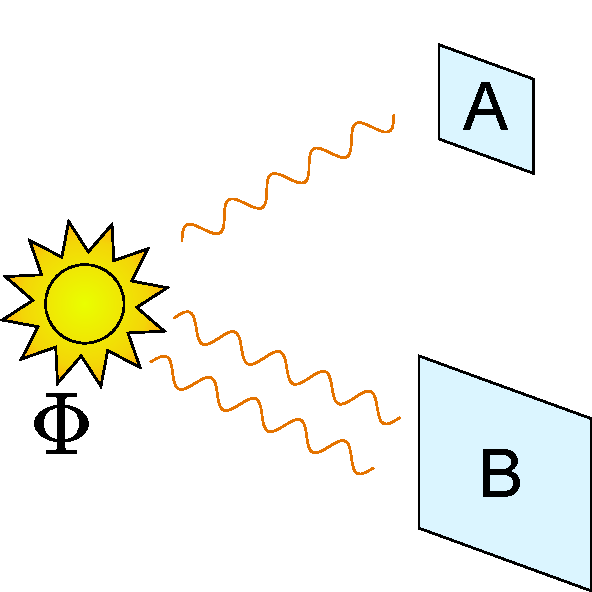
\includegraphics[width=0.5\textwidth]{images/irradiance.pdf}
\caption{Irradiance versus power. For the two surfaces $A$ and $B$, the received power $\Phi$ is the same, while the two irradiances $E_A$ and $E_B$ are different, as the area of $B$ is twice as the one of $A$.}
\label{fig:irradiance}
\end{figure}
 

\subsection{Intensity}
Intensity is defined as the differential radiant flux per differential solid angle:
$$
I(\vomega) = \frac{d \Phi}{d \omega}
\label{eq:i}
$$
It is measured in Watts per steradian [\si{\watt\per\steradian}] and it is indicated with the letter $I$. Intensity is often a misused term in the physics community, as it is used for many different quantities. Depending on the research community, intensity may refer to irradiance or even to radiance (see the following section). The definition given in \ref{eq:i} we use the most common definition given by the optics community.

\subsection{Radiance}
Radiance is arguably the most important quantity in image synthesis. It is defined precisely as the differential of the flux per solid angle per projected surface area, and it is measured in Watt per steradian per square meter [\si{\watt\per\steradian\meter\square}].
$$
L(\vomega) = \frac{d^2 \Phi}{d\omega dA \cos \theta}
$$
Where $\theta$ is the angle between the surface normal and the incoming ray of light (so that $\cos\theta = \vec{n} \cdot \vomega_i$). 

\begin{figure}[!ht]
\centering
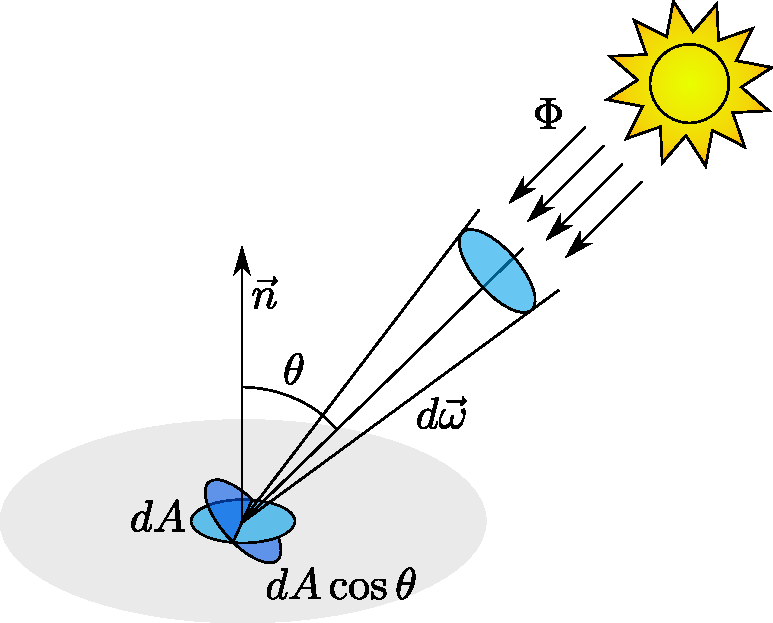
\includegraphics[width=0.7\textwidth]{images/radiance.pdf}
\caption{Radiance. The element of area $dA$ gets projected according to the angle $\theta = \cos^{-1}{\vec{n} \cdot \vomega}$. Then the incoming flux $\Phi$ gets divided by the projected area and by the solid angle subtended by it.}
\label{fig:radiance}
\end{figure}

Radiance has the important property of being constant along a ray of light. In addition, the sensibility of the human eye to light is directly proportional to the radiance. For a discussion on why radiance is related to the sensitivity of sensors and the human eye, see \cite{Cohen:1993:RRI:154731}.

All the other radiometric quantities can be derived from radiance:
\begin{equation}
\begin{split}
E &= \int_{2\pi} L_i(\vomega) \cos\theta \; d\omega \\
B &= \int_{2\pi} L_o(\vomega) \cos\theta \; d\omega \\
I(\vomega) &= \int_A L(\vomega) \cos\theta \; dA \\
\Phi &= \int_A \int_{2\pi} L(\vomega) \cos\theta \; d\omega dA
\end{split}
\label{eq:radiancederivation} 
\end{equation}
For simplicity of notation, the dependence from the point of incidence $\x$ has been dropped in equations \ref{eq:radiancederivation}. 

\subsection{Radiometric quantities for simple lights}

To help with the formulas used later in the report, we derive the standard radiometric quantities for the two simplest types of light, i.e. directional and point lights.
\begin{itemize}
	\item \textit{Directional lights} simulate very distant light sources, in which all the rays of light are parallel (e.g. sunlight). They are represented by a direction $\vomega_l$ and a constant radiance value, $L$. 
	\item \textit{Point lights} simulate lights closer to the observer. Isotropic point lights are represented by a position of the light $\x_l$ and a constant intensity $I$. Point lights have a falloff that depends on the inverse square law, i.e. the radiance diminishes with the square of the distance.
\end{itemize}

Table \ref{table:radio} shows different radiometric quantities evaluated for point and directional lights, for a surface point $\x$ with surface normal $\vec{n}$. 

\renewcommand{\arraystretch}{1.8}
\begin{table}[!ht]
    \centering
    \begin{tabularx}{0.95\textwidth}{|X|X|X|}
    \hline
    Quantity   & Directional light & Point light \\ \hline
    Cosine term       & $\cos\theta = \vec{n} \cdot \vomega_l$ & $\cos\theta = \frac{(\x - \x_l) \cdot \vec{n}}{|\x - \x_l|}$     \\ \hline
    $\Phi(\x)$ Flux       & $L\; \delta(\vec{\omega)}$                  & $4 \pi I$           \\ \hline
    $E(\x)$ Irradiance & $L \cos\theta $                 & $I \frac{\cos\theta}{|\x_l - \x|^2}$          \\ \hline
    $I(\x,\vomega)$ Intensity  & $L\; \delta(\vomega)$                 & $I$           \\ \hline
    $L(\x,\vomega)$ Radiance   & $L\; \delta(\vomega)$               & $\frac{I}{|\x_l - \x|^2}$           \\ \hline
    \end{tabularx}
\caption{Different radiometric values for simple light sources.}
\label{table:radio}
\end{table}

\section{Reflectance Functions}
After introducing the basic radiometric quantities, we still lack a way to describe light material interaction. More precisely, we need a way to relate the incoming and the outgoing radiance on a point of a chosen surface. 

\subsection{BRDF functions}
\label{sec:brdf}
One of the possible way to describe light-material interaction is by using a BDRF function \citep{Nicodemus:1992:GCN:136913.136929}, acronym for \emph{Bidirectional Reflectance Distribution Function}. The BRDF function $f(\x, \vomega_i, \vomega_o)$ is defined on one point $\x$ of the surface as the differential ratio between the exiting radiance and the irradiance:
\begin{equation}
f(\x, \vomega_i, \vomega_o) = \frac{d L_o(\x, \vomega_o)}{d E_i(\x, \vomega_i)} = \frac{d L_o(\x, \vomega_o)}{L_i(\x, \vomega_i) \cos\theta_i d \vomega_i}
\label{eq:brdf}
\end{equation}
The BRDF states that the incoming and the outgoing radiance are proportional, so that the energy hitting the material at the point $\x$ is proportional to the energy coming out from the point. BRDF functions have generally the following properties:
\begin{itemize}
	\item \emph{reciprocal}: for the Hemholtz reciprocity principle, a physics result that is also the basis of reverse path ray tracing \citep{Desolneux:2007:GTI:1557413}:
	$$
	f(\x, \vomega_i, \vomega_o) = f(\x, \vomega_o, \vomega_i)
	$$
	\item \emph{anisotropic}: if the surface changes orientation and $\vomega_i$ and $\vomega_o$ stays the same, the resulting BRDFs are different. So generally
	$$
	f(\x, \vomega_i, \vomega_o) \neq f(\x, R \vomega_o, R \vomega_i)
	$$
	where $R$ is a rotation matrix with arbitrary axis around the point $\x$.
	\item \emph{positive}, since the BRDF regulates the transport between two positive quantities (radiance, irradiance). 
	$$
	f(\x, \vomega_o, \vomega_i) \ge 0
	$$
	\item \emph{energy conserving}, so that the energy of the outgoing ray is no grater that the one of the incoming one 
	$$
	\int_{2\pi}  f(\x, \vomega_o, \vomega_i) \cos\theta_o d\vomega_o \le 1
	$$
\end{itemize}

By inverting equation \ref{eq:brdf}, we obtain the so-called \emph{reflectance equation}:
$$
L_o(\x, \vomega_o) = \int_{2\pi} f(\x, \vomega_i, \vomega_o) L_i(\x, \vomega_i) \cos\theta_i d\vomega_i
$$
Later we will use this equation as a starting point to obtain a formulation of the full rendering equation. The BRDF function has some limitations, being not able to account for all phenomena. For example, with a BRDF it is not possible to account for subsurface scattering, because it assumes the light enters and leaves the material at the same point. To model these phenomena, more complicated functions are needed, like the BSSRDF function described later in this chapter. 

\begin{figure}[!ht]
\centering
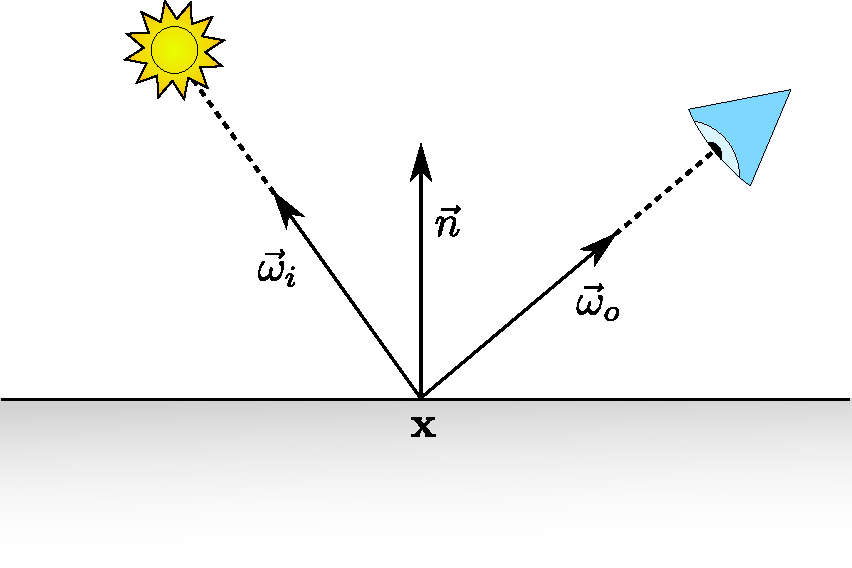
\includegraphics[width=0.8\textwidth]{images/brdf.pdf}
\caption{Setup for a BRDF. Note that the light enters and leaves the surface at the same point.}
\label{fig:brdf}
\end{figure}

\FloatBarrier 
\subsection{Examples of BRDF functions}
\begin{figure}
\centering
\subfloat[{Lambertian BRDF}]{
  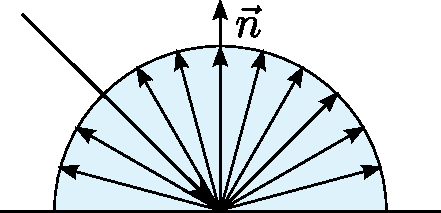
\includegraphics[width=0.4 \linewidth]{images/brdf_lambertian.pdf}
  \label{fig:lambertianbrdf}
}
\subfloat[{Mirror BRDF}]{
  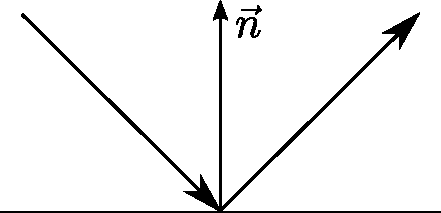
\includegraphics[width=0.4 \linewidth]{images/brdf_mirror.pdf}
  \label{fig:mirrorbrdf}
} \\
\subfloat[{Glossy BRDF}]{
  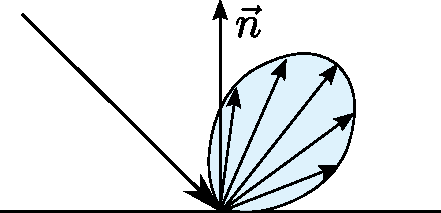
\includegraphics[width=0.4 \linewidth]{images/brdf_glossy.pdf}
  \label{fig:glossybrdf}
} 
\subfloat[{Combined BRDF}]{
  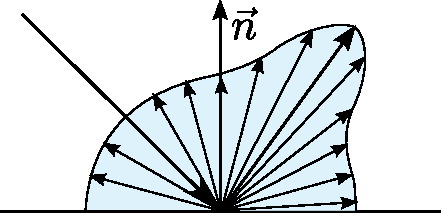
\includegraphics[width=0.4 \linewidth]{images/brdf_combined.pdf}
  \label{fig:combinedbrdf}
} 
\label{fig:brdfexamples}
\caption{Examples of BRDF functions. In this particular example, the three simple BRDFs can be evaluated separately and then combined in the more complex BRDF of Figure \ref{fig:combinedbrdf} in order to represent multiple effects.}
\end{figure}

There are many examples of BRDF functions in literature. In this section, in order to illustrate some examples, we will introduce three of them: the lambertian or diffuse BRDF, the specular or mirror BRDF and glossy BRDFs. For a detailed overview on BRDF functions, please refer to \citep{RTR3}.

\subsubsection{Lambertian BRDF}
In the lambertian BRDF, the incoming radiance is distributed equally in all directions, regardless of the incoming direction. To do this, the BRDF must be constant:
$$
f(\x, \vomega_i, \vomega_o) = k_d
$$
We can check that then the radiance is scattered equally in all directions by simple integration:

\begin{equation*}
\begin{split}
L_o(\x, \vomega_o) &= \int_{2\pi} f_d L_i(\x, \vomega_i) \cos\theta_i d\vomega_i \\
L_o(\x, \vomega_o) &= k_d \int_{2\pi} L_i(\x, \vomega_i) \cos\theta_i d\vomega_i \\
L_o(\x, \vomega_o) &= k_d \; E(\x) \\
\end{split}
\end{equation*}

The lambertian model is an ideal model, so very few material exhibit a lambertian diffusion, like unfinished wood or \emph{spectralon}, a synthetic material created in order to be as close as possible to a perfect lambertian material. Given its properties, spectralon is usually employed in calibrating radiance testing equipment. 

\subsubsection{Mirror BRDF}

Another simple kind of BRDF is the perfectly specular BRDF, or mirror BRDF. In this function, all the incoming radiance from one direction $\vomega_i$ is transferred towards the reflected direction $\vomega_r$, defined as $\vomega_r = \vomega_i - 2 (\vomega_i \cdot \vec{n}) \vec{n}$. The resulting BRDF is defined as follows:
$$
f(\x, \vomega_i, \vomega_o) = \frac{\delta(\vomega_o - \vomega_r)}{\cos\theta_i} 
$$
The function $\delta(\vomega)$ is a hemispheric delta function. Once integrated over a hemisphere, the function evaluates to one only for the vector $\vomega = \mathbf{0}$. Putting the BRDF into the reflectance equation gives the following outgoing radiance:
\begin{equation*}
L_o(\x, \vomega_o) = \begin{cases}
L_i(\x, \vomega_i)  &\text{if $\vomega_o = \vomega_r$}\\
0 &\text{otherwise}
\end{cases}
\end{equation*}
that is the expected result, as all the radiance is reflected into the direction $\vomega_r$.

\subsubsection{Glossy BRDFs}

As we can see from real life experience, rarely objects are completely diffuse or completely specular. These two models are idealized models, that represent an ideal case. So, to create a realistic BRDF model, we often need to combine the two terms and add an additional one, called glossy reflection.

The most used BRDF model used to model glossy reflections is based on microfacet theory \citep{Torrance:1992:TOR:136913.136924, Ashikmin:2000:MBG:344779.344814} and was first introduced by \citep{Blinn:1977:MLR:965141.563893}. In this theory, the surface of an object is modeled as composed of small mirrors. In one of its classical formulations, the BRDF is represented as:
$$
f(\x, \vomega_i, \vomega_o) = \frac{D G R}{4 \cos\theta_r \cos\theta_i} = \frac{G R}{4} \frac{(\vec{n}\cdot\vec{h})^s}{(\vec{n}\cdot\vec{r})(\vec{n}\cdot\vomega_i)}
$$
$D$ regulates how microfacets are distributed, and it is often modeled as $(\vec{n}\cdot\vec{h})^s$, where $\vec{h}$ is the half vector between the eye and the light, and $s$ is an attenuation parameter. $\vec{h}$ is defined as:
$$
\vec{h} = \frac{\vomega_o + \vomega_i}{\left\| \vomega_o + \vomega_i \right\|}
$$
$G$ accounts for the object self shadowing, while $R$ is the Fresnel reflection term (more details in Section \ref{sec:fresnel}).	$\vec{r}$ is the reflection vector as defined in the previous section. See Figure \ref{fig:glossysetup} on how the vectors for the glossy reflection - $\vec{n}$, $\vec{h}$ and $\vec{r}$ - are defined.


\begin{figure}[!ht]
\centering
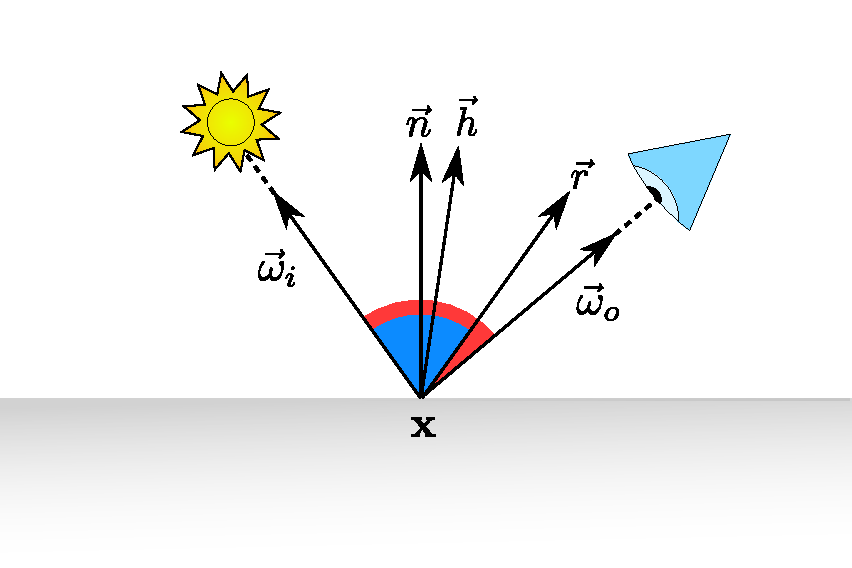
\includegraphics[width=0.7\textwidth]{images/glossy_setup.pdf}
\caption{Glossy vectors for microfacet theory. The blue angles are the same for the reflection vector, the red ones are the same for the half vector.}
\label{fig:glossysetup}
\end{figure}
 
Various alternative definitions exist for the $D$ and $G$ function, varying among the literature. Other glossy models not based on microfacet theory do exist as well \citep{RTR3}. 

\subsection{The rendering equation}

Given the reflectance equation, it is possible to generalize it in order to model all the lighting in an environment (global illumination). In fact, the described reflectance equation is a suitable candidate to represent a full global illumination equation, but it does not account for two important factors. 

The first factor are emissive surfaces. We need to add an emissive radiance term $L_e(\x, \vomega)$ that models the amount of radiance that a point is emitting in a certain direction. This is useful to model light sources, without introducing a separate equation. We note that point lights have a singularity: they emit infinite radiance on the point where they are placed.

The second factor is that the reflectance equation accounts only for direct illumination. In general, we want to include also light that bounced onto another surface before reaching the current surface. To model this, we can replace the $L_i$ term in the reflectance equation with another term $L_r$ that accounts for light coming from another surface. This term can be usually modeled as the product of the radiance of the light plus a visibility function $V(\x)$.

Accounting for all the described factors, we reach one formulation of the rendering equation \citep{Kajiya:1986:RE:15886.15902}:
$$
L_o(\x, \vomega_o) = L_e(\x, \vomega) + \int_{2\pi} f(\x, \vomega_i, \vomega_o) L_i(\x, \vomega_i) V(\x) \cos\theta_i d\vomega_i
$$
This form of the rendering equation is still not completely general, since it is based on a BRDF, to it comes with the same limitations (no subsurface scattering effects or wavelength-changing effects like iridescence). We will extend the rendering equation in order to account for these phenomena later on in this chapter.

\subsection{Fresnel equations}
\label{sec:fresnel}

Until now, on the described BRDF models, we did consider only the reflected part of the radiance. When a beam of light coming from direction $\vomega_i$ hits a surface, only part of the incoming radiance gets reflected, while another part gets refracted into the material. As we can see from Figure \ref{fig:fresnelsetup}, we obtain the two vectors $\vomega_r$ and $\vomega_t$, the reflected and refracted vector, defined as follows \citep{Kay:1979:TCS:965103.807438}:
\begin{equation*}
\begin{split}
\vomega_r &= \vomega_i - 2 (\vomega_i \cdot \vec{n}) \vec{n} \\
\vomega_t &= \eta ((\vomega_i \cdot \vec{n}) \vec{n} - \vomega_i) - \vec{n} \sqrt{1 - \eta^2 (1 - (\vomega_i \cdot \vec{n}) ^ 2)}
\end{split}
\end{equation*}
\begin{figure}[!ht]
\centering
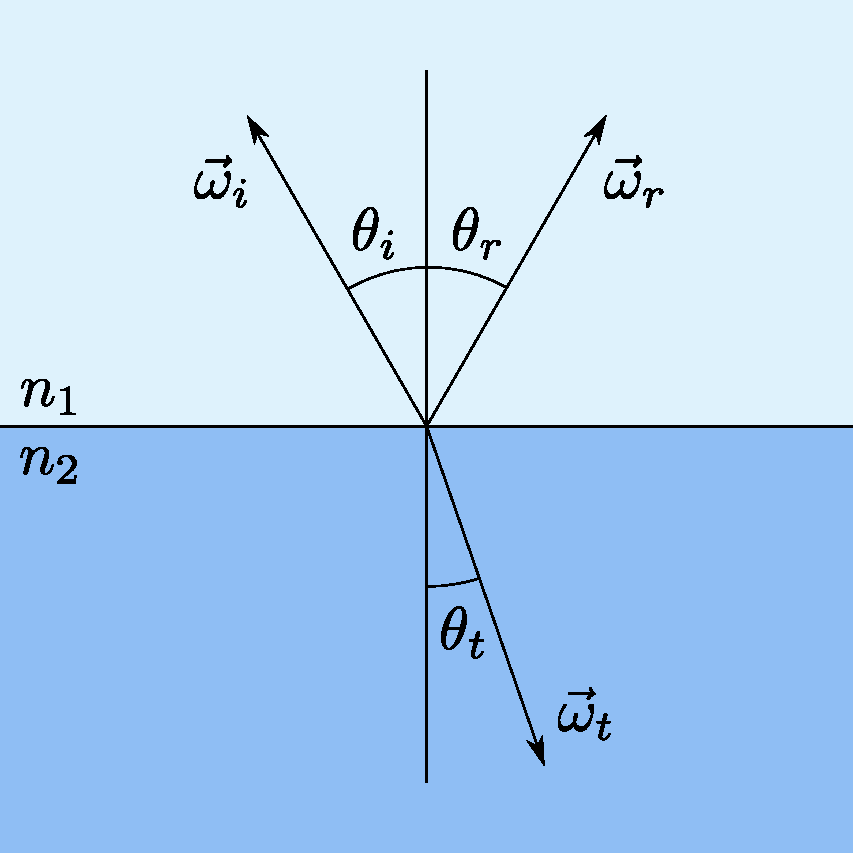
\includegraphics[width=0.5\textwidth]{images/fresnelsetup.pdf}
\caption{Reflected and refracted vector on mismatching indices of refraction.}
\label{fig:fresnelsetup}
\end{figure}
Where $\eta = \frac{n_1}{n_2}$ is the relative index of refraction between the two materials. With this setup, illustrated in Figure \ref{fig:fresnelsetup}, we can use a solution to Maxwell's equations for wave propagation to describe the radiant flux. In particular, we can tell which part of the power propagates in the reflected and refracted direction respectively. The coefficients that describe this subdivision of the power are called \emph{Fresnel coefficients} \citep{ob:bornwolf}. The coefficients are different according to the polarization of the incoming light (parallel or perpendicular), so there are two for reflection ($R_s$, $R_p$) and two for transmission ($T_s$, $T_p$).
\begin{equation*}
\begin{split}
R_s(\eta,\vomega_i) &= \left|\frac{\eta \cos\theta_i - \cos\theta_t} {\eta \cos\theta_i + \cos\theta_t}\right|^2 \\
R_p(\eta,\vomega_i) &= \left|\frac{\eta \cos\theta_t - \cos\theta_i} {\eta \cos\theta_t + \cos\theta_i}\right|^2\\
T_s(\eta,\vomega_i) &= \eta \ \frac{ \cos\theta_t}{ \cos\theta_i} \left|\frac{2 \cos\theta_i}{\eta \cos\theta_i + \cos\theta_t}\right|^2 \\
T_p(\eta,\vomega_i) &= \eta \ \frac{ \cos\theta_t}{ \cos\theta_i} \left|\frac{2 \cos\theta_i}{\eta \cos\theta_t + \cos\theta_i}\right|^2
\end{split}
\end{equation*}
In most computer graphics applications (and this is reasonable for most of the real-world lights), we assume that the two polarizations are equally mixed. So, we will use the coefficient $R = \frac{R_s + R_p}{2}$ and $T = \frac{T_s + T_p}{2}$ in our calculations. Note that $R + T = 1$, so the overall energy is conserved.

\subsection{BSSRDF functions and generalized rendering equation}
\begin{figure}
\centering
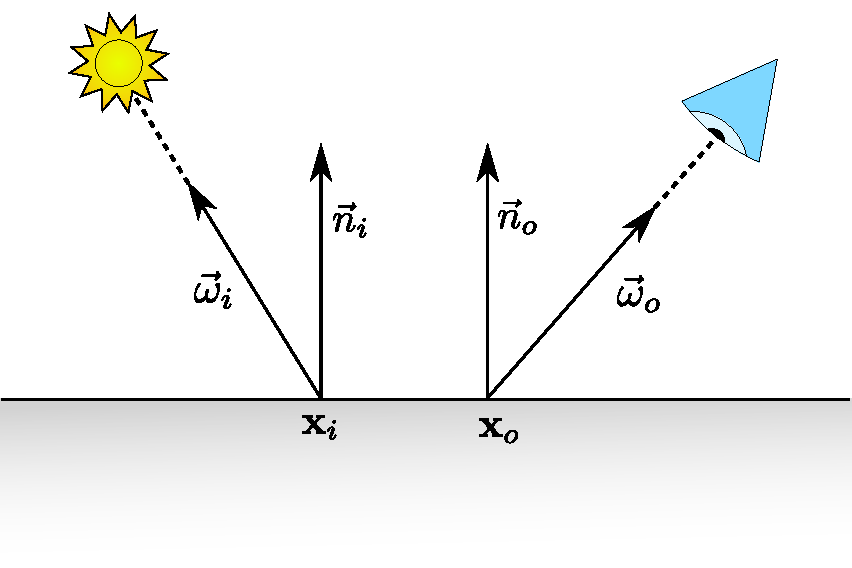
\includegraphics[width=0.8 \linewidth]{images/bssrdf} 
\caption{BSSRDF setup. As we compare it to the one of Figure \ref{fig:brdf}, we can see that the light enters and leaves the surface at two different points.}
\label{fig:bssrdf}
\end{figure}

As we anticipated in Section \ref{sec:brdf}, the BRDF theory that was introduced before is not accurate in predicting the behavior for all materials, since BRDF models assume that the light enters and leaves the material in the same point. While this assumption holds true for a wide range of material, like metal or plastic, it poorly describes translucent materials, that exhibit a consistent amount of light transport under the surface. 

In order to describe light transport in this material, we introduce a function, called BSSRDF \citep{Nicodemus:1992:GCN:136913.136929}, acronym for \emph{Bidirectional Subsurface Scattering Reflectance Distribution Function}. This function extends the concept of BRDF to account for two separate points. The BSSRDF is usually indicated with a capital $S$. We define the BRDF as the ratio between the incoming flux in a point $\x_i$ from the direction $\vomega_i$ and the outgoing radiance in \emph{another} point $\x_o$ on direction $\vomega_o$:
$$
S(\x_i, \vomega_i, \x_o, \vomega_o) = \frac{d L_o(\x_o,\vomega_o)}{d \Phi_i(\x_i,\vomega_i)} = \frac{d L_o(\x_o,\vomega_o)}{d E_i(\x_i,\vomega_i) d A_i} = \frac{d L_o(\x_o,\vomega_o)}{L_i(\x_i,\vomega_i) \cos \theta_i d\vomega_i d A_i}  
$$
As we can see, the BSSRDF is similar to the BRDF, apart from a additional derivation in the area domain. Once we rearrange this equation, we can obtain an updated reflectance equation for the BSSRDF:
$$
L_o(\x_o,\vomega_o) = \int_A \int_{2\pi} S(\x_i, \vomega_i, \x_o, \vomega_o) L_i(\x_i,\vomega_i) \cos \theta_i d\vomega_i d A_i
$$
We can immediately see that the new reflectance equation accounts for light scattering between two points, but this generality comes with a price. In fact, it adds a order of magnitude of complexity, since now the BSSRDF needs to be integrated twice, once on the whole surface and once on the normal hemisphere.

As we did for the BRDF, we can further extend the reflectance equation to further include visibility and emission, giving an extended form of the rendering equation \citep{Jensen:2001:PMS:383259.383319}. 
\begin{equation}
L_o(\x_o,\vomega_o) = L_e(\x_i,\vomega_i) + \int_A \int_{2\pi} S(\x_i, \vomega_i, \x_o, \vomega_o) L_i(\x_i,\vomega_i) V(\x) (\vec{n} \cdot \vomega_i) d\vomega_i d A_i
\label{eq:bssrdfeq}
\end{equation}
From now on, by `rendering equation' in this report we will mean the one in equation \ref{eq:bssrdfeq}. 

\section{Light transport and subsurface scattering}
\FloatBarrier
\begin{figure}
\centering
\subfloat[{Emission}]{
  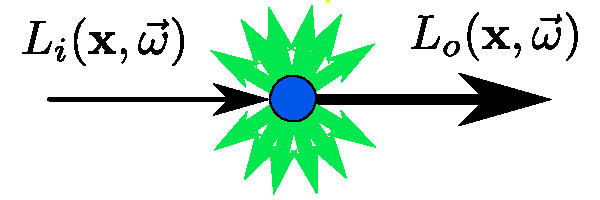
\includegraphics[width=0.5 \linewidth]{images/transport_emission.pdf}
  \label{fig:emission}
}
\subfloat[{Absorption}]{
  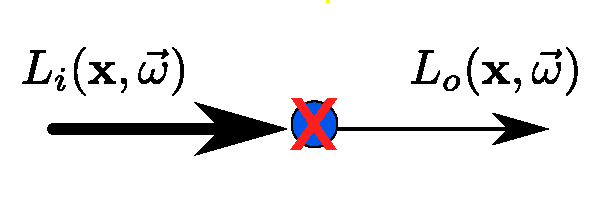
\includegraphics[width=0.5 \linewidth]{images/transport_absorption.pdf}
  \label{fig:absorption}
} \\
\subfloat[{Out Scattering}]{
  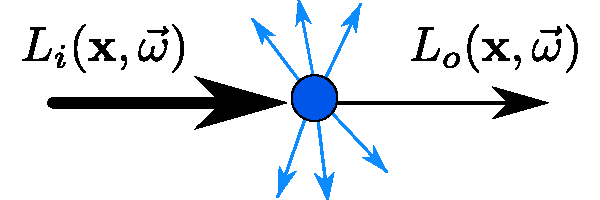
\includegraphics[width=0.5 \linewidth]{images/transport_outscattering.pdf}
  \label{fig:outscattering}
} 
\subfloat[{In Scattering}]{
  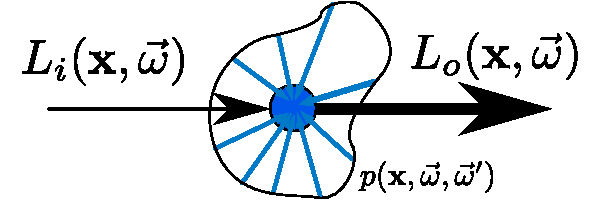
\includegraphics[width=0.5 \linewidth]{images/transport_inscattering.pdf}
  \label{fig:inscattering}
} 
\label{fig:transport}
\end{figure}

When we derive our models for lighting, in general we assume that the light is traveling in vacuum. This assumption holds for light that is propagating though the air (which is assimilable to vacuum), but once we relax it, more variables should be taken into consideration. Objects through which light travels are referred as \emph{participating media}. In this chapter, we will derive and consider an alternative formulation of the rendering equation for light traveling into participating media, called \emph{radiative transfer equation} \citep{Chandrasekar:1950:RT}.

When a beam of light travels through an object, various phenomena occur. A photon on the beam can be either being absorbed (disappear), scattered (change direction) or emitted (appear). These phenomena can be uniform throughout the material (homogeneous materials), as in solid materials like wax or leaves, or be not uniform (heterogeneous materials), like in smoke or clouds.

We will briefly describe all three mentioned effects, then combine them to compose the radiative transfer equation. The purpose is to describe how radiance varies along a beam of light with direction $\vomega$. This directional derivative is indicated as:
$$
(\vec{\nabla} \cdot \vomega) L(\x, \vomega) = \frac{\partial L_x}{\partial x} \vomega_x + \frac{\partial L_y}{\partial y} \vomega_y + \frac{\partial L_z}{\partial z} \vomega_z
$$ 

\subsection{Emission}
Emission is the natural property of the materials to emit light, i.e. to generate photons that add to the existing ones passing through the material. The effect is generally generated by chemical processes emitting photons (as in fireflies), by natural black-body radiation emission in the visible spectrum (such as in a star like the sun or in incandescent bulbs), or by other radiation that changes its wavelength into the visible spectrum.

In the directional 3D derivative, the variance in emission is modeled as a constant depending only on the current position and direction:
$$
(\vec{\nabla} \cdot \vomega) L(\x, \vomega) = \epsilon(\x, \vomega)
$$
This means that emission increases linearly along the body: if the beam travels a distance $d$ within the medium, $d \cdot k$ photons are emitted. Emission is generally isotropic, not depending on the direction ($ \epsilon(\x, \vomega) =  \epsilon(\x)$).

\subsection{Absorption}
Absorption is a property of materials that describes a simple physical phenomenon: a photon, traveling though the material, hits one atom of the material. The energy carried by the photon is then absorbed by the atom, augmenting its kinetic energy. This directly translates in an increase of heat in the material. Usually, a certain percentage of the photons that hit the atoms is absorbed per unit length. Then, if $k$ is the percentage of the photons absorbed in a meter, after one meter the original radiance will become $k \cdot L_i$, then $k^2 \cdot L_i$, etc.

If we write this phenomena as a differential equation, we get after a distance $d$ a radiance reduction of $k^d = e^{-\sigma_a d}$, that leads to the following 3D directional derivative:
$$
(\vec{\nabla} \cdot \vomega) L(\x, \vomega) = -\sigma_a(\x,\vomega) L(\x, \vomega)
$$
$\sigma_a$ is referred as the \emph{absorption coefficient}. Also this coefficient is generically isotropic, and constant for homogenous materials.

\subsection{Out-scattering}
Out scattering is the radiance lost due to scattering. The scattering phenomenon happens when photons are deflected away from the current direction $\vomega$.  As in the previous case, the phenomena is modeled as a percentage of the radiance lost per unit length. So the loss due to out-scattering is modeled as:
$$
(\vec{\nabla} \cdot \vomega) L(\x, \vomega) = -\sigma_s(\x,\vomega) L(\x, \vomega)
$$
$\sigma_s$ is referred as the \emph{scattering coefficient}. We note that in this case we are not interested in which direction the photons are actually going. That will be accounted in the in-scattering term of another point in the material.

\subsection{In-scattering}
Given some loss due to some of the photons changing direction, there will be some of them that from other scattering events will change to the $\vomega$ direction. We need then to discover the number of photons that comes from all the other directions. To do this, we integrate the incoming radiance from all directions in the point $\x$. This quantity, similar to irradiance, in an infinite medium is called \emph{fluence}, and indicated as $\phi$:
$$
\phi(\x) = \int_{4\pi} L(\x,\vomega') d\omega'
$$
Fluence should be then averaged over the entire sphere, yielding $\frac{\phi}{4\pi}$ as a normalization factor. This quantity then is then multiplied by the scattering coefficient, because only some photons on average scatter towards the current point. This results in:
\begin{equation}
(\vec{\nabla} \cdot \vomega) L(\x, \vomega) = \sigma_s(\x) \frac{1}{4 \pi} \int_{4\pi} L(\x,\vomega') d\omega'	
\label{eq:inscatter}
\end{equation}
However, equation \ref{eq:inscatter} assumes that radiance scatters equally in all directions. This is not usually the case, and the $\frac{1}{4 \pi}$ term needs to be replaced by a probability distribution function that describes how the photons scatter in the medium. This function is called \emph{phase function}, and indicated as $p(\x, \vomega, \vomega')$. In the actual models its integral on the hemisphere is often used as a parameter, called \emph{mean cosine} ($g$):
$$
g(\x) = \int_{4 \pi} p(\x, \vomega, \vomega') \vomega \cdot \vomega' d \omega'
$$
This term indicates the general direction of the scattering in the material. If positive, the scattering is prevalent along the beam (forward scattering), if negative is prevalent in the opposite direction (backward scattering). If zero, the scattering is isotropic, i.e. equal in all directions.

So, the final 3D equation for in-scattering, accounting for the phase function, is as follows:
\begin{equation*}
(\vec{\nabla} \cdot \vomega) L(\x, \vomega) = \sigma_s(\x) \int_{4\pi} p(\x, \vomega, \vomega') L(\x,\vomega') d\omega'	
\end{equation*}

\subsection{Final formulation of the radiative transfer equation}
Combining emission, absorption, scattering described in the previous sections, we reach the final formulation of the radiative transfer equation (RTE):
\begin{equation}
(\vec{\nabla} \cdot \vomega) L(\x, \vomega) =   -\sigma_t(\x) L(\x, \vomega) + \epsilon(\x) + \sigma_s(\x) \int_{4\pi} p(\x, \vomega, \vomega') L(\x,\vomega') d\omega'
\label{eq:rte}
\end{equation}
Where the two reducing term, scattering and absorption, have been combined together in $\sigma_t = \sigma_a + \sigma_s$, called the \emph{extinction coefficient}.


\subsection{The diffusion approximation}
The radiative transfer equation \ref{eq:rte} is a integro-differential equation with many degrees of freedom. As we stated in Chapter \ref{chap:previous}, there are rendering techniques that numerically solve the equation in order to obtain a realistic result. However, analytical methods tend to use some approximations of the RTE, that hold well given specific conditions. The \emph{diffusion approximation} \citep{books/daglib/0093591} is one of these approximations, and it is still widely used today since its introduction in the computer graphics community by \citep{raey}. 

The assumption under the diffusion approximation is that given a physical medium, the number of scattering events is so high that the beam of light quickly becomes isotropic. Each one of the scattering events blurs the light distribution, and as a result the distribution becomes more uniform as the number of scattering events increases. This has been proven to be a reasonable assumption even for highly anisotropic light sources (e.g. a focused laser beam) and phase functions.

When using the diffusion approximation, instead of using the extinction coefficient $\sigma_t$, we account for the contribution from the phase function by using the so-called \emph{reduced extinction coefficient} $\sigma_t'$. It is defined as $\sigma_t' = \sigma_a + \sigma_s'$, with $\sigma_s' = \sigma_s (1 - g)$. $\sigma_s'$ Is called \emph{reduced scattering coefficient}. The converse of the reduced extinction coefficient is called \emph{mean free path} and represents the average distance that light travels in the medium before being absorbed or scattered.

The rationale behind this reduced coefficient is that a highly forward scattering material is virtually indistinguishable from a not-scattering material. So, for highly forward scattering materials ($g \approx 1$) the scattering coefficients reduce to zero. For highly backward scattering materials ($g \approx -1$), the scattering is accounted for twice as for an isotropic material (see table \ref{table:coefficients}).

\renewcommand{\arraystretch}{1.8}
\begin{table}[!ht]
    \centering
    \begin{tabularx}{0.95\textwidth}{|X|X|X|X|}
    \hline
    Coefficient   & Backward\linebreak Scattering \linebreak $(g \approx -1)$ & Isotropic \linebreak\linebreak $(g \approx 0)$ & Forward \linebreak Scattering \linebreak $(g \approx 1)$ \\ \hline
    $\sigma_s'$   & $2 \sigma_s$ & $\sigma_s$ & 0   \\ \hline
    $\sigma_t'$   & $\sigma_a + 2 \sigma_s$ & $\sigma_a + \sigma_s$ &  $\sigma_a$  \\ \hline
    \end{tabularx}
\caption{Explicit scattering coefficients for different kinds of materials.}
\label{table:coefficients}
\end{table}

We leave to \cite{books/daglib/0093591} and \cite{Jensen:2001:PMS:383259.383319} for the algebraic details of the calculation. Once we solve the diffusion equation, we obtain the following formula for $\phi(\x)$, the fluence of light in an infinite scattering medium.
$$
\phi(\x) = \frac{\Phi}{4\pi D} \frac{e^{\sigma_{tr} r}}{r}
\label{eq:dasimple}
$$
We recall that $\phi(\x) = \int_{4\pi}L(\x,\vomega) d\vomega$. $r = \|\x\|$ is the distance from the point to the light source. The two coefficients $D$ and $\sigma_{tr}$ are called \emph{diffusion coefficient} and \emph{transmission coefficient} respectively. The two coefficients are defined as follows:
\begin{equation*}
\begin{split}
D &= \frac{1}{3 \sigma_t'} \\
\sigma_{tr} &= \sqrt{3 \sigma_a \sigma_t'} = \sqrt{\frac{\sigma_a}{D}}
\end{split}
\end{equation*}
This is the equation describe light propagation in an infinite medium, i.e. no surface interaction is considered. In order to derive an actual BSSRDF model from the diffusion approximation, \emph{boundary conditions} must be considered. Jensen \cite{Jensen:2001:PMS:383259.383319} derived an analytical model starting from this approximation of the RTE, while Frisvad \cite{IMM2013-06646} uses a higher order diffusion approximation of the RTE. The two models are explained in the following sections.

\subsection{Standard dipole model}
 
The first model we describe is due to \cite{Jensen:2001:PMS:383259.383319}. It it usually referred in literature as \emph{Jensen dipole model} or \emph{Standard dipole model}. In their original paper, the authors used the diffusion approximation for light in an infinite medium. Starting from that, they derive an approximation that holds for light in a semi-infinite medium, i.e. light traveling in void hitting a planar slab of a translucent material.

As a boundary condition, we take the light coming \emph{out} of the material. Light coming out of the material has a initial fluence $\phi_0$. We assume then that the fluence decays linearly until a distance $z = 2 A D$ from the surface, where it becomes zero. See \cite{Donner:2006:TRI:1236937} for the full derivation. $D$ is the diffusion coefficient, while $A$ is a corrective term that accounts for mismatching indices of refraction:
\begin{equation}
\begin{split}
A &= \frac{1 + F_{dr}}{1 - F_{dr}} \\
F_{dr} &= \int_{2\pi} R(\eta, \vec{n} \cdot \vomega)  (\vec{n} \cdot \vomega) d \vomega
\end{split}
\end{equation}
Where $R$ is the Fresnel reflection term as defined in Section \ref{sec:fresnel}, and $\eta = n_1 / n_2$ is the relative refraction index. The Fresnel reflectance integral $F_{dr}$ is usually approximated with an analytical expression:
$$
F_{dr} = -\frac{1.440}{\eta^2} + \frac{0.710}{\eta} + 0.668 + 0.0036 \eta
$$
Given the boundary condition, we can then model the subsurface scattering in a point $\x_o$ with two small sources on the point, a configuration called a \emph{dipole}. One source is placed beneath the surface, called the \emph{real source}, while the other one is mirrored above the surface, called \emph{virtual source}. The first source actually models the subsurface scattering effect, while the second one reduces the first in order to account for the boundary conditions and the extrapolation boundary. Refer to Figure \ref{fig:jensen} for a visual detail on the setup.

\begin{figure}[!ht]
\centering
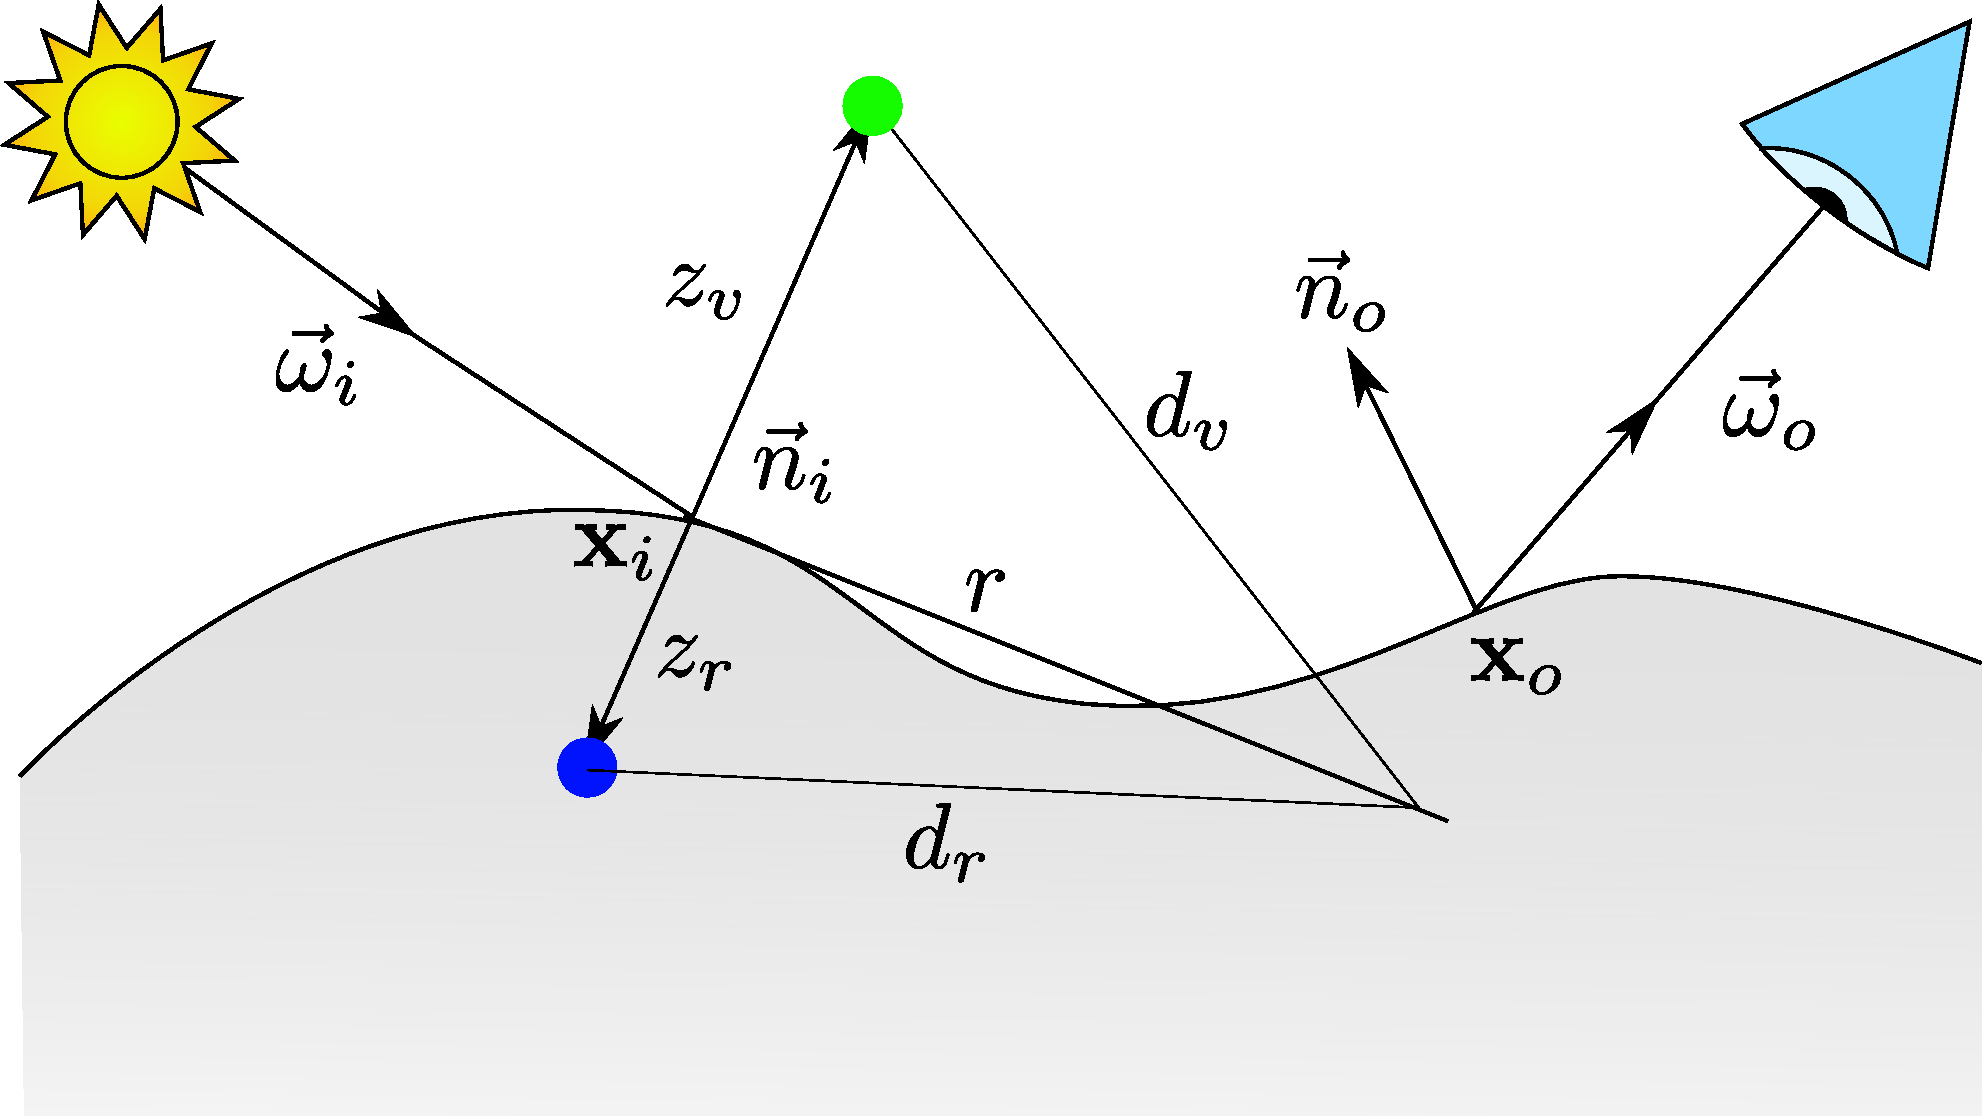
\includegraphics[width=\textwidth]{images/jensen.pdf}
\caption{Setup for the standard dipole model.}
\label{fig:jensen}
\end{figure}

The real source is placed one mean free path beneath the surface, at $z_r = 1 / \sigma_t'$, while the virtual one is placed symmetrically according to the boundary conditions, ad a distance $z_v = z_r + 4 A D$. From $z_r$ and $z_v$ we can calculate the distances $d_r$ and $d_v$ from the entrance point $\x_i$. Given $r = \|\x_o -\x_i\|$, we obtain:
\begin{equation*}
\begin{split}
d_r &= \sqrt{z_r^2 + r^2} \\
d_v &= \sqrt{z_v^2 + r^2}
\end{split}
\end{equation*}
Given these constraints, we obtain an equation for the BSSRDF in a semi infinite medium:
$$
S_d(\x_i,\vomega_i,\x_i,\vomega_o) = \frac{\alpha'}{4 \pi^2} \left[\frac{z_r (1 + \sigma_{tr} d_r) \; e^{-\sigma_{tr} d_r}}{d_r^3} + \frac{z_v (1 + \sigma_{tr} d_v) \; e^{-\sigma_{tr} d_v}}{d_v^3} \right]
$$
Where $\alpha' = \sigma_s' / \sigma_t'$ is called \emph{reduced albedo}.

The model so far described was intended to model only the multiple scattering BSSRDF term, $S_d$. In order to obtain the full BSSRDF $S$, a single scattering term $S^{(1)}$ must be added. Moreover, we need to add as well the two Fresnel transmission terms, one for the incoming and one for the outgoing radiance. There are in literature many approaches to model single scattering, that are out of the scope of this report. The final BSSRDF equation for the standard dipole model then becomes:
$$
S(\x_i, \vomega_i, \x_o, \vomega_o) = T(\eta,\vomega_i) S_d(\x_i, \vomega_i, \x_o, \vomega_o) T(\eta,\vomega_o) + S^{(1)}(\x_i, \vomega_i, \x_o, \vomega_o)
$$
\cite{Jensen:2001:PMS:383259.383319} in their original paper describes some corrections that need to be done to the model in order to make it work with generic surfaces, and on how to account for extensions like texture support. We will not describe these extensions here, remanding to the original paper for a detailed description.

\subsection{Directional dipole model}
 
Various evolutions to the standard dipole model have been proposed throughout the years. In this chapter, we will introduce the BSSRDF approximation called \emph{directional dipole}, proposed by \cite{IMM2013-06646}. In the standard dipole model, in fact, the diffusive part of the BSSRDF depends only on the distance between the point of incidence and the point of emergence, that is $S_d(\x_i, \vomega_i, \x_o, \vomega_o) = S_d(\|\x_o - \x_i\|)$. 

The directional dipole model, based on the diffusion approximation, accounts for the direction of the incoming light in its calculations, in order to model the scattering effects more precisely. Moreover, the model, instead of splitting the BSSRDF in a multiple and single scattering term, splits the BSSRDF into a diffusive term $S_d$ and a term $S_{\delta E}$, called \emph{reduced intensity}, that can be computed using the delta-Eddington approximation\cite{delta}. The final BSSRDF thus becomes:
$$
S(\x_i, \vomega_i, \x_o, \vomega_o) = T(\eta,\vomega_i) (S_d(\x_i, \vomega_i, \x_o) + S_{\delta E}(\x_i, \vomega_i, \x_o, \vomega_o)) T(\eta,\vomega_o)
\label{eq:bssrdfgen}
$$
Where $T$ are the Fresnel transmission coefficients for the incoming and outgoing directions. We note also that the diffusive part of the BSSRDF does not depend on the outgoing direction $\vomega_o$. 

\textbf{Diffusive BSSRDF}
The diffusive part of the directional dipole model uses a first-order approximation of the RTE, that for a point light in an infinite medium gives the following fluence:
$$
\phi(\x_o, \theta) = \frac{\Phi}{4\pi D} \frac{e^{\sigma_{tr} r}}{r} \left( 1 + 3D\frac{1 + \sigma_{tr} r}{r}\cos\theta\right)
\label{eq:daa}
$$
Where $D$ and $\sigma_{tr}$ are the two scattering coefficients defined beforehand, $r = \|\x_o\|$ and 
$$
\cos \theta = \frac{\x \cdot \vomega_{12}}{r}
$$
Where $\vomega_{12}$ is the refracted vector as defined in Section \ref{sec:fresnel}. Comparing \ref{eq:daa} with equation \ref{eq:dasimple}, we can see that we introduced a new term that depends on the angle $\theta$ between the refracted incoming light vector and the vector connecting incidence and emergence. 

\begin{figure}[!ht]
\centering
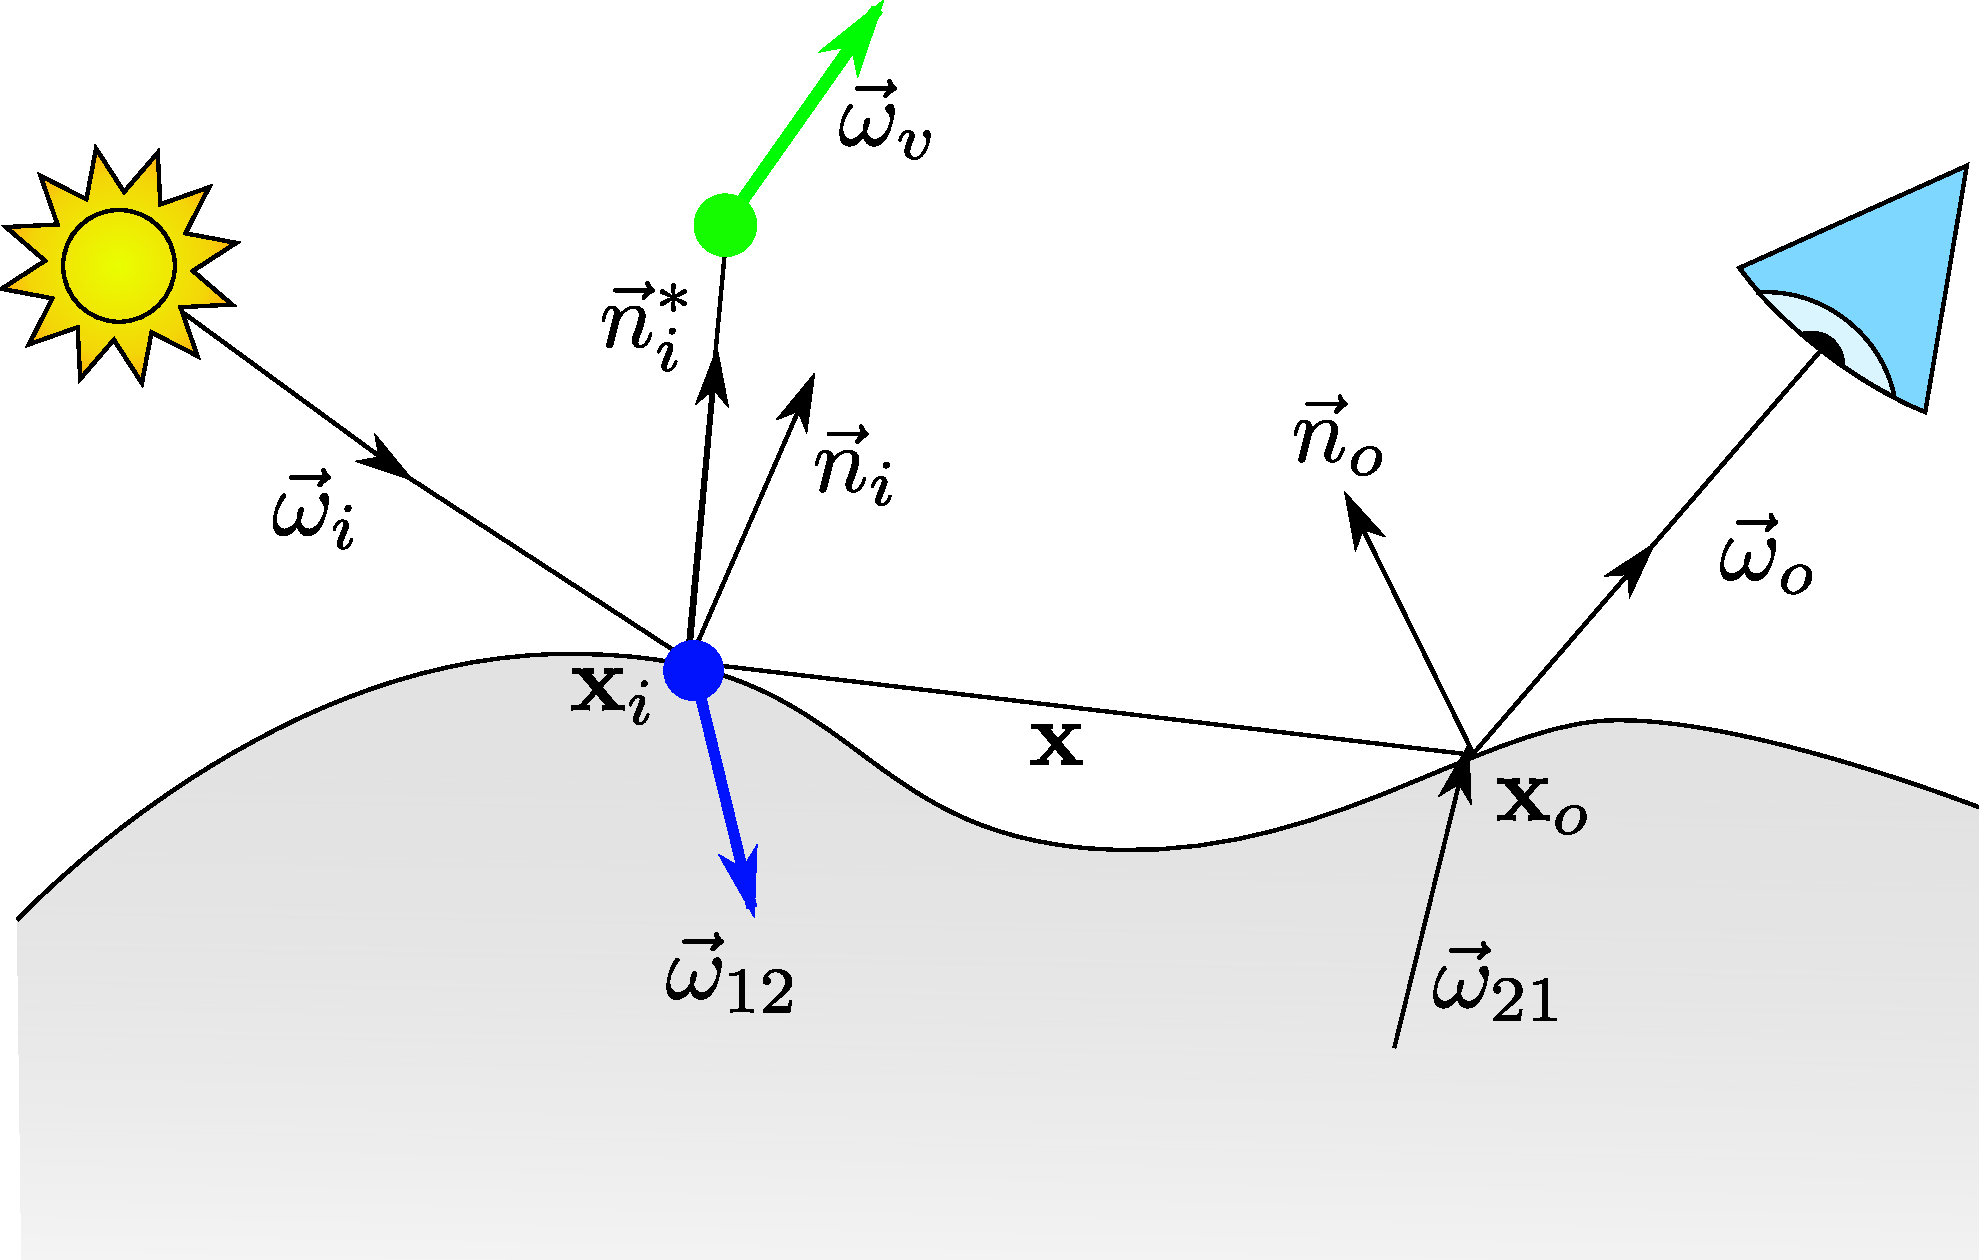
\includegraphics[width=0.9\textwidth]{images/jeppe.pdf}
\caption{Setup for the directional dipole model.}
\label{fig:jeppe}
\end{figure}

Using the diffusion approximation, we can first establish a relationship between the radiant exitance $M(\x_o)$ and the diffusive BSSRDF $S'_d$ in an infinite medium:
$$
\frac{d M(\x_o)}{d \Phi_i(\x, \vomega_i)} = T(\eta, \vomega_i) S'_d(\x_i, \vomega_i, \x_o) \; 4\pi\csinv 
\label{eq:m2}
$$
Where $\csinv$ is related to the integral on the hemisphere of the fresnel coefficients. Using the definition of radiant exitance and inserting inside the classical diffusion approximation, we reach the diffusion formulation of the radiant exitance:
$$
M(\x_o) = \cs \phi(\x_o) + \ce D \vec{n}_o \cdot \nabla \phi(\x_o)
\label{eq:m3}
$$
Again, $\cs$ and $\ce$ are two terms that are related to the integration of the fresnel coefficients. Combining the three equations \ref{eq:daa}, \ref{eq:m2} and \ref{eq:m3}, we reach the final form for our diffusive BSSRDF in an infinite medium:
\begin{equation}
\begin{split}
&S'_d(\x, \vomega_{12}, r) = \frac{1}{4\csinv} \frac{1}{4\pi^2} \frac{e^{-\sigma_{tr} r}}{r^3} \\
&\bigg[ \cs \left(\frac{r^2}{D} + 3 (1 + \sigma_{tr} r ) \x \cdot \vomega_{12} \right) - \\
&-\ce \bigg(3D (1 + \sigma_{tr} r) \; \vomega_{12} \cdot \vec{n}_o - \\ 
&-\left( (1 + \sigma_{tr} r) + 3D \frac{3(1 + \sigma_{tr} r ) + (\sigma_{tr} r)^2}{r^2}  \x \cdot \vomega_{12} \right)  \x \cdot \vec{n}_o \bigg) \bigg] 
\end{split}
\end{equation}

\begin{mybox}
\begin{center}\textbf{Fresnel integrals}\end{center}
The two terms $\cs$ and $\ce$ originally come from integrating the outgoing Fresnel transmittance over the whole outgoing hemisphere, weighted with a cosine term. The two functions are defined as follows: 
\begin{equation}
\begin{split}
\cs &= \frac{1}{4\pi} \int_{2\pi} T(\eta,\vomega) (\vec{n}_o \cdot \vomega) d \vomega \\
\ce &= \frac{3}{4\pi} \int_{2\pi} T(\eta,\vomega) (\vec{n}_o \cdot \vomega)^2 d \vomega \\
\end{split}
\end{equation}

These two integrals can be rearranged in order to express them in terms of reflectance instead of transmittance, recalling $R = 1 - T$.
\begin{equation}
\begin{split}
\cs &= \frac{1}{4\pi} \left( \pi - \int_{2\pi} R(\eta,\vomega) (\vec{n}_o \cdot \vomega) d \vomega \right) = \frac{1}{4}(1 - 2 C_1)\\
\ce &= \frac{3}{4\pi} \left(\frac{2\pi}{3} - \int_{2\pi} R(\eta,\vomega) (\vec{n}_o \cdot \vomega) d \vomega \right) = \frac{1}{2}(1 - 3 C_2) \\
\end{split}
\end{equation}

Even with this rearrangement the integrals cannot be expressed in closed form. \cite{D'Eon:2011:QMR:1964921.1964951} use a convenient polynomial approximation for the two coefficients $C_1$ and $C_2$, expressed as:

$$
2 C_1\approx 
\begin{cases}			
	+0.919317-3.4793\eta + 6.75335\eta^2 -7.80989\eta^3\\ \hspace{3.2cm}+4.98554\eta^4-1.36881\eta^5& \eta < 1 \\
	-9.23372 + 22.2272\eta-20.9292\eta^2 + 10.2291\eta^3\\ \hspace{3.2cm}-2.54396\eta^4 + 0.254913\eta^5 & \eta \geq 1

\end{cases}
$$
$$
3 C_2 \approx
\begin{cases}
0.828421-2.62051\eta + 3.36231\eta^2 -1.95284\eta^3\\ \hspace{3cm}+ 0.236494\eta^4 + 0.145787\eta^5 & \eta < 1 \\
-1641.1 + \frac{135.926}{\eta^3} - \frac{656.175}{\eta^2} + \frac{1376.53}{\eta} + 1213.67\eta \\ \hspace{3cm} -568.556\eta^2 + 164.798\eta^3\\ \hspace{3cm} -27.0181\eta^4 + 1.91826\eta^5 & \eta \geq 1.
\end{cases}
$$
\end{mybox}

\textbf{Boundary conditions}

As the name implies, also for the directional dipole we model the boundary conditions on the material interface using a dipole. In this case, however, instead of using two point light sources, we use two ray sources, a real and a virtual one. As in the standard dipole, the source is displaced towards the normal of a distance $d_e$. In the case of the standard dipole, we use $2D$, that becomes $2 A D$ in the case of mismatching indices of refraction on the interface. In the case of the directional dipole, we use 
$$
d_e = \frac{2.131 D}{\sqrt{\alpha'}}
$$ 
Where we recall $\alpha' = \sigma_s' / \sigma_t'$ as the reduced albedo. This result have been proven \citep{ntt} to be consistent with numerical simulations of the RTE. In addition, the $A$ term is modified using the hemispheric Fresnel integrals:
$$
A(\eta) = \frac{1 - \ce}{2 \cs}
$$
As the standard dipole, the directional dipole assumes a semi-infinite medium given the previous boundary conditions. In order to relax this assumptions, we need to further extend the model in order to reduce undesired effects. One first modification proposed by \cite{IMM2013-06646} is to use a modified tangent plane defined by the normal $\vec{n}_i^*$ to mirror the real source towards the mirror light source, instead of the obvious one defined by $\vec{n}_i$. We define the modified normal as follows:
$$
\vec{n}_i^* = 
\begin{dcases} 
\vec{n}_i & \text{for}\ \x_o = \x_i \\
\frac{\x_o - \x_i}{\|\x_o - \x_i\|} \times \frac{\vec{n}_i \times (\x_o - \x_i)}{\|\vec{n}_i \times (\x_o - \x_i)\|} & \text{otherwise}
\end{dcases}
$$
Another important modification is the distance to the real source. In the standard dipole, we used $d_r = \sqrt{z_r^2 + r^2}$, with $z_r = 1 / \sigma_t'$, which is the average distance a photon travels within the material before being absorbed or scattered. The problem of this definition is that it introduces a singularity in $r = 0$. Moreover, the standard dipole becomes fairly imprecise when $r$ is small, overestimating the overall effect. In order to avoid these problems, \cite{IMM2013-06646} proposed a more complicated definition of $d_r$ that matches simulation of transport theory more closely. For the details, see Appendix B in the original paper. $d_r$ is defined as follows, recalling $\sigma_t = \sigma_s + \sigma_a$:
$$
d_r^2 = \begin{dcases}
r^2 + D \mu_0 (D \mu_0 - 2 d_e \cos \beta) & \mu_0 \geq 0 \  \text{(frontlit)}\\
r^2 + \frac{1}{(3 \sigma_t)^2} & \mu_0 < 0 \ \text{(backlit)}
\end{dcases}
$$
Where $\mu_0 = - \vomega_{12} \cdot \vec{n}_o$ is an indicator if the point $\x_o$ is frontlit or backlit. $\beta$ is a geometry term that is evaluated as:
$$
\cos \beta = - \sqrt{\frac{r^2 - (\x \cdot \vomega_{12})^2}{r^2 + d_e^2}}
$$
Combining all the corrections seen so far, we can write the final form of our BSSRDF model, that is a combination of the real source term minus the virtual source term:
$$
S_d(\x_i, \vomega_i, \x_o) = S'_d(\x_o - \x_i, \vomega_{12}, d_r) - S'_d(\x_o - \x_v, \vomega_{v}, d_v)
$$
Where the extra coefficients for the virtual source are defined as follows:
\begin{equation*}
\begin{split}
x_v &= x_i + 2 A d_e \vec{n}_i^* \\
\vomega_v &= \vomega_{12} - 2 (\vomega_{12} \cdot \vec{n}_i^*) \vec{n}_i^* \\
d_v &= \|x_o - x_v\|
\end{split}
\end{equation*}
The directional dipole model described in this chapter, gives a better result that the standard dipole, at the extra price of additional calculations. In particular, the model improves the previous one for highly forward scattering materials, where it is sensibly closer to the path traced result. The final goal of this thesis is to provide a real-time implementation of it. Given this theoretical introduction, in the next section we will describe our contribution in order to breakdown the problems and the issues of a real-time implementation.

\begin{figure}
\centering
\subfloat[{Standard dipole}]{
  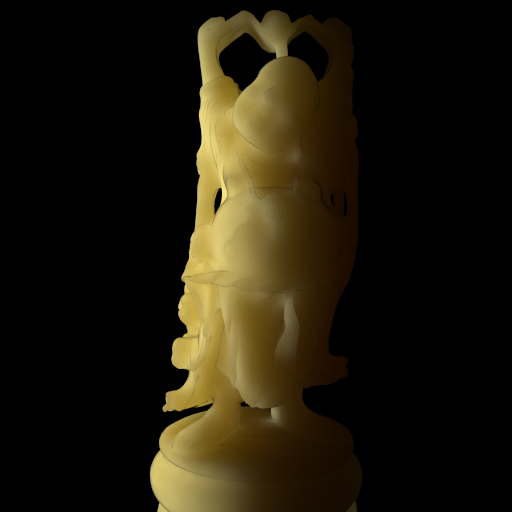
\includegraphics[width=0.5 \linewidth]{images/gamma_potato_buddha_dipole.png}
}
\subfloat[Directional Dipole]{
  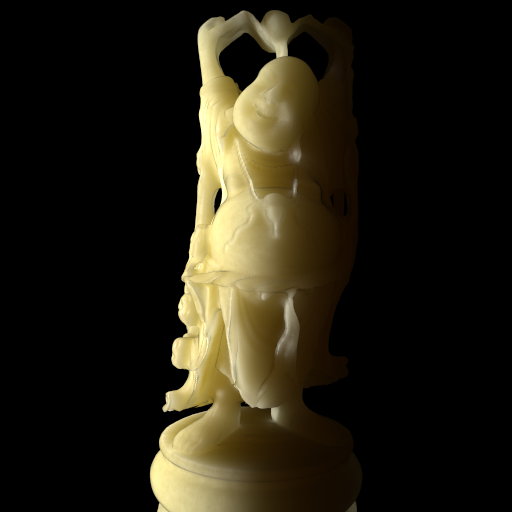
\includegraphics[width=0.5 \linewidth]{images/gamma_potato_buddha_dir.png}
}
\caption{Comparison of the standard and the directional dipole model, for a Stanford Happy Buddha made of potato, with a side directional light. We can see that  the directional dipole is able to capture finer details and provide a generally less flat appearance than the standard one.}
\label{fig:bssrdfcomparison}
\end{figure}
